\tikzset{
  estilo nodos/.style={
      node distance=2.5cm,
      estado/.style={circle, draw, minimum size=1cm, inner sep=0pt},
      proba/.style={-latex, thin, bend left=20pt},
      every node/.style={font={\tiny}},
    },
  add flechas/.code={
      \draw[proba] (0) to node[above] {rec.} (1);
      \draw[proba] (1) to node[above] {rec.} (2);
      \draw[proba] (2) to node[above] {$\dots$} (dots.north west);
      \draw[proba] (dots.north east) to node[above] {$\dots$} (n-2);
      \draw[proba] (n-2) to node[above] {rec.} (n-1);
      \draw[proba] (n-1) to node[above] {rec.} (n);
    },
}
\begin{enunciado}{\ejercicio[ComplexityQuest]}
  \textit{ComplexityQuest}

  Calcule la complejidad de un algoritmo que utiliza $T(n)$ pasos para una entrada de tamaño $n$,
  donde $T$ cumple:
  \begin{enumerate}[label=\arabic*)]
    \begin{multicols}{3}
      \item $T(n) = T(n - 2) + 5$
      \item $T(n) = T(n - 1) + n$
      \item $T(n) = T(n - 1) + \sqrt{n}$
      \item $T(n) = T(n - 1) + n^2$
      \item $T(n) = 2T(n - 1)$

      \item $T(n) = T(n/2) + n$
      \item $T(n) = T(n/2) + \sqrt{n}$
      \item $T(n) = T(n/2) + n^2$
      \item $T(n) = 2T(n/2) + n^2$

      \item $T(n) = 2T(n-4)$
      \item $T(n) = 2T(n/2) + \log(n)$
      \item $T(n) = 3T(n/4)$
      \item $T(n) = 3T(n/4) + n$
    \end{multicols}
  \end{enumerate}
\end{enunciado}

\parrafoDestacado{
  En los ejercicios donde $\magenta{a} = 1 \ytext \blue{b} = 1$ el \textit{Teorema Maestro}
  \ul{no está bien} definido. En la demo, se usá como hipótesis que $\frac{\magenta{a}}{\blue{b}} > 1$.
}

\parrafoDestacado[\atencion]{
  Si puedo evitar usar de forma explícita el \textit{Teorema Maestro} lo voy a hacer. Te \red{sugiero}
  intentar hacerlos sin esa fórmula fea también, porque sino no entendés un choto de lo que está pasando
  con la complejidad.
}

\parrafoDestacado[\calculator]{
  Voy a estar usando esta identidad:
  $
    \cajaResultado{
      a^{\log_b(c)} = c^{\log_b(a)}
    }
  $.
  Se muestra fácil aplicando $\log_a()$ en ambos miembros
  $$
    \begin{array}{rcl}
      a^{\log_b(c)} = c^{\log_b(a)}
       & \Sii{aplico $\log_a()$}[ambos miembros] &
      \log_b(c) \cdot \ob{\log_a(a)}{\magenta{1}} = \log_b(a) \cdot \green{\log_a(c)}   \\
       & \Sii{cambio}[de base]                   &
      \log_b(c) \cdot \magenta{1} = \log_b(a) \cdot \green{\frac{\log_b(c)}{\log_b(a)}} \\
       & \Sii{\red{!}}                           &
      \log_b(c) \igual{\checkmark} \log_b(c)                                            \\
    \end{array}
  $$
}

\parrafoDestacado{
  \it
  ¿No sabés cambiar la base de un $\log$? Aprendelo ayer. Hacete un favor y eliminá ruido cognitivo
  de tu vida, once and for all.
}

\bigskip

\begin{enumerate}[label=\arabic*)]
  \item No puedo usar el \textit{Teorema Maestro}. Hay que calcular a mano. El árbol de recursión tiene una sola rama.

        $$
          T(n) =
          \llave{ccl}{
            5 & \text{si} & n = 0\\
            T(n - 2) + 5 & \text{si} & n > 0
          }
        $$
        Tengo un costo en cada \textit{subproblema} de $5$:
        $$
          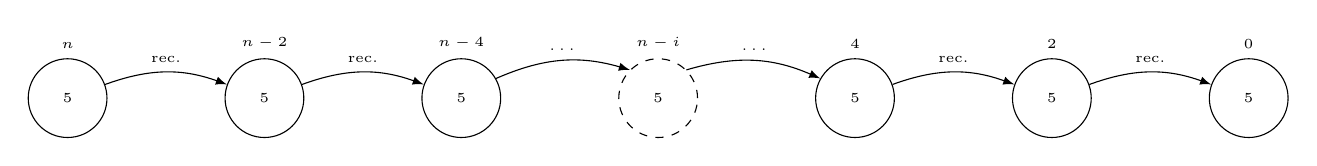
\begin{tikzpicture}[estilo nodos]
            \node[estado, label=above:{$n$}] (0) {$5$};
            \node[estado, right of=0, label=above:{$n-2$}] (1) {$5$};
            \node[estado, right of=1, label=above:{$n-4$}] (2) {$5$};
            \node[estado, right of=2, label={$n-i$}, dashed] (dots) {$5$};
            \node[estado, right of=dots, label=above:{$4$}] (n-2) {$5$};
            \node[estado, right of=n-2, label=above:{$2$}] (n-1) {$5$};
            \node[estado, right of=n-1, label=above:{$0$}] (n) {$5$};

            \draw[proba] (0) to node[above] {rec.} (1);
            \draw[proba] (1) to node[above] {rec.} (2);
            \draw[proba] (2) to node[above] {$\dots$} (dots.north west);
            \draw[proba] (dots.north east) to node[above] {$\dots$} (n-2);
            \draw[proba] (n-2) to node[above] {rec.} (n-1);
            \draw[proba] (n-1) to node[above] {rec.} (n);
          \end{tikzpicture}
        $$
        \parrafoDestacado{
          \textit{
            ¿Cuál es la altura o longitud de este \textit{árbol}?}

          \textit{
            Será la cantidad de veces, $k$, que tenga que hacer recurrencia hasta llegar al \textit{caso base}:
          }
        }
        $$
          T(n - 2k) \igual{?} T(0) \sisolosi n - 2k = 0 \sisolosi \boxed{k = n/2}
        $$

        El costo usando $n_p$ par o $n_i$ impar, de tal manera que habría $k = n/2$ llamados recursivos (el $O$ se come los casos borde).
        El \textit{running time} del algoritmo es el costo de resolver cada subproblema, 5 en este caso, por la cantidad de llamados, $n/2$
        en este caso:
        $$
          \textstyle
          T(n) = \sumatoria{i = 1}{k} 5 \igual{\red{!}} 5 \cdot \frac{n}{2} \en \Theta(n)
        $$

        \bigskip

        En este caso los llamados recursivos dominan el \textit{running time}:
        $$
          \cajaResultado{
            \textstyle
            T(n) \en \Theta(n)
          }
        $$

        %2
  \item Parecido al anterior.
        $$
          T(n) =
          \llave{ccl}{
            1 & \text{si} & n = 0\\
            T(n - 1) + n & \text{si} & n > 0
          }
        $$
        Tengo un costo para resolver cada \textit{subproblema} de $n$:
        $$
          \begin{tikzpicture}[estilo nodos, add flechas]
            \node[estado, label=above:{$n$}] (0) {$n$};
            \node[estado, right of=0, label=above:{$n-1$}] (1) {$n-1$};
            \node[estado, right of=1, label=above:{$n-2$}] (2) {$n-2$};
            \node[estado, right of=2, label={$n-i$}, dashed] (dots) {$n-i$};
            \node[estado, right of=dots, label=above:{$2$}] (n-2) {$2$};
            \node[estado, right of=n-2, label=above:{$1$}] (n-1) {$1$};
            \node[estado, right of=n-1, label=above:{$0$}] (n) {$0$};
          \end{tikzpicture}
        $$
        \parrafoDestacado{
          \textit{
            ¿Cuál es la altura o longitud de este \textit{árbol}?}

          \textit{
            Será la cantidad de veces, $k$, que tenga que hacer recurrencia hasta llegar al \textit{caso base}:
          }
        }
        $$
          T(n - k) \igual{?} T(0) \sii n - k = 0 \sii \boxed{k = n}
        $$
        Tengo un total de $n$ iteraciones:
        $$
          \textstyle
          T(n) = \sumatoria{i = 1}{n} i = \frac{n \cdot (n+1)}{2} \en \Theta(n^2)
        $$

        \bigskip

        El \textit{running time $T$} está dominado por la llamada recursiva:
        $$
          \cajaResultado{
            \textstyle
            T(n) \en \Theta(n^2)
          }
        $$

        %3
  \item Parecido al anterior.
        $$
          T(n) =
          \llave{rcl}{
            1 & \text{si} & n = 0\\
            T(n - 1) + \sqrt{n} & \text{si} & n > 0
          }
        $$

        Tengo un costo, \textit{running time}, para resolver cada \textit{subproblema} de $\sqrt{n}$:
        $$
          \begin{tikzpicture}[estilo nodos, add flechas]
            \node[estado, label=above:{$n$}] (0) {$\sqrt{n}$};
            \node[estado, right of=0, label=above:{$n-1$}] (1) {$\sqrt{n-1}$};
            \node[estado, right of=1, label=above:{$n-2$}] (2) {$\sqrt{n-2}$};
            \node[estado, right of=2, label={$n-i$}, dashed] (dots) {$\sqrt{n-i}$};
            \node[estado, right of=dots, label=above:{$2$}] (n-2) {$\sqrt{2}$};
            \node[estado, right of=n-2, label=above:{$1$}] (n-1) {$\sqrt{1}$};
            \node[estado, right of=n-1, label=above:{$0$}] (n) {$\sqrt{0}$};
          \end{tikzpicture}
        $$
        Tengo un total de $n$ llamados:
        $$
          \textstyle
          T(n) =
          \sumatoria{i = 1}{n} \sqrt{i} =
          \sumatoria{i = 1}{n} i^{\frac{1}{2}} \taa{\red{!!}}{}{\approx}
          \integral{1}{n} i^{\frac{1}{2}} di =
          \frac{2}{3} i^{\frac{3}{2}} \barrow{1}{n} =
          \frac{2}{3} (n^{\frac{3}{2}} - 1)
          \en \Theta(n^{\frac{3}{2}})
        $$

        \bigskip

        El llamado recursivo domina el \textit{running time} nuevamente.
        $$
          \cajaResultado{
            T(n) \en \Theta(n^\frac{3}{2})
          }
        $$

        %4
  \item
        Tengo un total de $n$ iteraciones. Similar a los ejercicios anteriores, sumar todas las contribuciones me da:
        $$
          \textstyle
          T(n) = \sumatoria{i = 1}{n} i^2 \approx
          \integral{1}{n} i^2 di =
          \frac{1}{3} i^3 \barrow{1}{n} =
          \frac{1}{3} (n^3 - 1)
          \en \Theta(n^3)
        $$

        \bigskip
        El llamado recursivo domina el \textit{running time} nuevamente.
        $$
          \cajaResultado{
            T(n) \en \Theta(n^3)
          }
        $$

        %5
  \item\label{ej7-itemII}
        Por fin empiezan a aparecer \textit{más cantidad de subproblemas} en cada iteración, así le pone un poquito de sal.
        $$
          T(n) =
          \llave{ccl}{
            0 & \text{si} & n = 0 \\
            2T(n - 1)& \text{si} & n > 0
          }
        $$

        Si no tengo un costo para resolver subproblemas ($f(n) = 0$) la complejidad depende solo del llamado recursivo.
        Entonces el \textit{running time, complejidad o como más te guste}
        es igual a contar la cantidad de nodos del árbol recursivo, la cantidad de llamadas que hace la función.

        Estoy partiendo al problema en 2 problemas de (casi) igual tamaño, así que puedo esperar que la complejidad explote con $n$.
        Tengo un árbol de $n$ niveles:

        \forestset{
        nivel/.style={label={[below left, xshift=-3mm]:{\tiny \red{ nivel: $#1 \to$}}}},
        binary tree/.style={
            for tree={
                scale=0.6,
                circle, draw, minimum size=1cm,
                math content,
                s sep=.3cm, l sep=.2cm,
              },
          }
        }

        $$
          \begin{forest}
            binary tree,
            [0, nivel={0}
                  [0, nivel={1}
                      [0,  nivel={2}
                          [\cdots
                            [0, nivel={n}]
                            [0]
                          ]
                          [\cdots
                            [0]
                            [0]
                          ]
                      ]
                      [0
                          [\cdots
                            [0]
                            [0]
                          ]
                          [\cdots
                            [0]
                            [0]
                          ]
                      ]
                  ]
                  [0
                      [0
                          [\cdots
                            [0]
                            [0]
                          ]
                          [\cdots
                            [0]
                            [0]
                          ]
                      ]
                      [0
                          [\cdots
                            [0]
                            [0]
                          ]
                          [\cdots
                            [0]
                            [0]
                          ]
                      ]
                  ]
              ]
          \end{forest}
        $$
        Para calcular el costo total, hay que calcular la cantidad de nodos. En el nivel 1, tengo $2^1$ nodos, en el nivel $i$ tengo $2^i$:
        $$
          T(n) =
          \sumatoria{i = 0}{n} 2^i
          \igual{\red{!}}
          \frac{2^{n+1} - 1}{2 - 1} \en \Theta(2^n)
        $$
        El \textit{running time} está claramente dominado por los llamados recursivos:
        $$
          \cajaResultado{
            T(n) \en \Theta(2^n)
          }
        $$

        %6
  \item El árbol recursivo tiene una sola rama.
        El \texttt{input} se parte a la mitad en cada iteración, por lo tanto voy a tener un árbol de altura $\log_2(n)$:
        $$
          T(n) =
          \llave{ccl}{
            1 & \text{si} & n = 1 \\
            T(n/2) + n& \text{si} & n > 1
          }
        $$

        $$
          \begin{tikzpicture}[estilo nodos, add flechas, etiqueta/.style={label=above:{size: $#1$}}]
            \node[estado, etiqueta={n}] (0) {$n$};
            \node[estado, right of=0, etiqueta={n/2} ] (1) {$n/2$};
            \node[estado, right of=1, etiqueta={n/4} ] (2) {$n/2^2$};
            \node[estado, right of=2] (dots) {$\cdots$};
            \node[estado, right of=dots, label=above:{$4$}] (n-2) {$4$};
            \node[estado, right of=n-2, label=above:{$2$}] (n-1) {$2$};
            \node[estado, right of=n-1, label=above:{$1$}] (n) {$1$};
          \end{tikzpicture}
        $$

        \parrafoDestacado{
          \textit{
            ¿Cuál es la altura o longitud de este \textit{árbol}?
          }

          \textit{
            Será la cantidad de veces, $k$, que tenga que hacer recurrencia hasta llegar al caso base:
          }
        }
        $$
          \textstyle
          T(\frac{n}{2^k}) \igual{?} T(1) \sii \frac{n}{2^k} = 1 \sii \boxed{k = \log_2(n)}
        $$

        Por ejemplo:
        Si $n = 32$, pasados 5 llamados(en la misma rama) se llega al caso base, dado que $\log_2(32) = 5$
        $$
          \begin{array}{rcl}
            T(n)  =                \sumatoria{i = 1}{\log_2n} \frac{n}{2^i}
             & \igual{\red{!}} &
            n \cdot \sumatoria{i = 1}{\log_2n} (\frac{1}{2})^i                        \\
             & =               &
            n \cdot  \frac{(\frac{1}{2})^{\log_2(n) + 1} - \frac{1}{2}}{-\frac{1}{2}} \\
             & =               &
            n \cdot  (-2) \cdot (\frac{1}{2n} - \frac{1}{2})                          \\
             & =               &
            n - 1                                                                     \\
             & \en             &
            O(n)
          \end{array}
        $$

        La sumatoria geométrica con razón menor a 1, aporta muy poco, porque \textit{decrece muy rápido asintóticamente}, es por eso que el costo
        de resolver cada \textit{subproblema} ($f(n) = n$) domina la complejidad.
        $$
          \cajaResultado{
            T(n) \en \Theta(n)
          }
        $$

        %7
  \item  Parecido al anterior.

        El árbol de recursión va a dar una geométrica de razón menor a 1, por lo tanto la complejidad tiene que estar dominada
        por el costo de resolver los subproblemas:

        $O(\sqrt{n})$ porque el \textit{input} se achica exponencialmente rápido y $\paratodo k>0, n^k$ asintóticamente le va a ganar.

        \textit{...Anyways}
        $$
          T(n) =
          \llave{ccl}{
            1 & \text{si} & n = 1 \\
            T(n/2) + \sqrt{n}& \text{si} & n > 1
          }
        $$
        El triste árbol de recursión va a tener una sola rama y una altura (¿longitud?) de $\log_2(n)$.
        $$
          \begin{tikzpicture}[estilo nodos, add flechas, etiqueta/.style={label=above:{size: $#1$}}]
            \node[estado, etiqueta={n}] (0) {$\sqrt{n}$};
            \node[estado, right of=0, etiqueta={n/2} ] (1) {$\sqrt{n/2}$};
            \node[estado, right of=1, etiqueta={n/4} ] (2) {$\sqrt{n/2^2}$};
            \node[estado, right of=2, etiqueta={n/2^i}] (dots) {$\sqrt{n/2^i}$};
            \node[estado, right of=dots, label=above:{$4$}] (n-2) {$\sqrt{4}$};
            \node[estado, right of=n-2, label=above:{$2$}] (n-1) {$\sqrt{2}$};
            \node[estado, right of=n-1, label=above:{$1$}] (n) {$\sqrt{1}$};
          \end{tikzpicture}
        $$

        Sumando las contribuciones:
        $$
          \begin{array}{rcl}
            \sumatoria{i = 1}{\log_2(n)} \sqrt{\frac{n}{2^i}} & \igual{\red{!}} & \sqrt{n} \cdot \sumatoria{i = 1}{\log_2(n)} (\frac{1}{\sqrt{2}})^i \\
                                                              & =               &
            \sqrt{n} \cdot \frac{(\frac{1}{\sqrt{2}})^{\log_2(n) + 1} - \frac{1}{\sqrt{2}}}{\frac{1}{\sqrt{2}} - 1}                                  \\
                                                              & =               &
            \sqrt{n} \cdot \frac{\frac{1}{\sqrt{n}} \cdot  \frac{1}{\sqrt{2}} - \frac{1}{\sqrt{2}}}{\frac{1 - \sqrt{2}}{\sqrt{2}}}                   \\
                                                              & =               &
            \frac{1 - \sqrt{n}}{1-\sqrt{2}}                                                                                                          \\                                                                     \\
                                                              & \en             & \Theta(\sqrt{n})
          \end{array}
        $$

        Como era lo esperado, las llamadas recursivas decrecen muy rápido por lo tanto domina el \textit{running time}
        la complejidad de $f(n)$, el costo de resolver cada subproblema.

        $$
          \cajaResultado{
            T(n) \en \Theta(\sqrt{n})
          }
        $$

        %8
  \item Idem anterior, esto tiene que dar $\Theta(n^2)$ por la misma razón.

        $$
          T(n) =
          \llave{ccl}{
            0 & \text{si} & n = 0 \\
            T(n/2) + n^2& \text{si} & n > 0
          }
        $$
        El triste árbol de recursión va a tener una sola rama y una altura de $\log_2(n)$.
        $$
          \begin{tikzpicture}[estilo nodos, add flechas, etiqueta/.style={label=above:{size: $#1$}}]
            \node[estado, etiqueta={n}] (0) {$n^2$};
            \node[estado, right of=0, etiqueta={n/2} ] (1) {$(n/2)^2$};
            \node[estado, right of=1, etiqueta={n/4} ] (2) {$(n/2^2)^2$};
            \node[estado, right of=2] (dots) {$(n/2^i)^2$};
            \node[estado, right of=dots, label=above:{$2$}] (n-2) {$(1/4)^2$};
            \node[estado, right of=n-2, label=above:{$1$}] (n-1) {$(1/2)^2$};
            \node[estado, right of=n-1, label=above:{$0$}] (n) {$0$};
          \end{tikzpicture}
        $$

        Sumando las contribuciones:
        $$
          \textstyle
          \sumatoria{i = 1}{\log_2(n)} (\frac{n}{2^i})^2 \igual{\red{!}}
          n^2 \cdot
          \sumatoria{i = 1}{\log_2(n)} (\frac{1}{4})^i =
          n^2 \cdot
          \frac{(\frac{1}{4})^{\log_2(n) + 1} - \frac{1}{4}}{\frac{1}{4} - 1} \igual{\red{!}}
          n^2 \cdot
          \frac{(\frac{1}{n^2}) \cdot \frac{1}{4} - \frac{1}{4}}{\frac{1}{4} - 1} \igual{\red{!}}
          \frac{1}{2} \cdot (n^2 - 1) \en \Theta(n^2)
        $$

        Era esperado, la complejidad de resolver cada subproblema, domina la complejidad total del algoritmo:
        $$
          \cajaResultado{
            T(n) \en \Theta(n^2)
          }
        $$

        %9
  \item\label{ej7-itemI}
        Acá aparece una función con 2 llamados recursivos, esto cambia un poco el cálculo. El árbol tiene 2 ramas principales ahora
        que se van bifurcando en cada iteración. El árbol va a tener $\log_2(n)$ niveles.
        $$
          T(n) =
          \llave{ccl}{
            1 & \text{si} & n = 1 \\
            2T(n/2) + n^2 & \text{si} & n > 1
          }
        $$
        $$
          \forestset{
          nivel/.style={label={[below left, xshift=-7pt, yshift=-1pt]:{\red{\tiny size \texttt{input}: $#1 \to$}}}},
          binary tree/.style={
              for tree={
                  scale=0.6,
                  circle, draw, minimum size=1cm,
                  math content,
                  s sep=.3cm, l sep=.2cm,
                },
            }
          }
          \begin{forest}
            binary tree,
            [n^2, nivel={n}
            [(\frac{n}{2})^2, nivel={n/2}
              [\cdots
                [1, nivel={1}]
                [1]
              ]
              [\cdots
                [1]
                [1]
              ]
            ]
            [(\frac{n}{2})^2
            [\cdots
            [1]
            [1]
            ]
            [\cdots
            [1]
            [1]
            ]
            ]
            ]
          \end{forest}
        $$

        Sumando las contribuciones:

        Se puede estimar la contribución total. Por ejemplo en el \textit{nivel 0} hay un sólo
        vértice (la raíz), que tiene una contribución de $n^2$, en el \textit{nivel $1$} la contribución es:
        $$
          \textstyle
          (\frac{n}{2})^2 + (\frac{n}{2})^2 = 2(\frac{n}{2})^2 = \frac{1}{2} n^2.
        $$
        La contribución se redujo a la mitad.

        En el \textit{nivel $2$} será:
        $$
          \textstyle
          (\frac{n}{4})^2 + (\frac{n}{4})^2 + (\frac{n}{4})^2 + (\frac{n}{4})^2 = 4(\frac{n}{4})^2 = \frac{1}{4} n^2.
        $$
        Volvió a disminuir a la mitad
        \parrafoDestacado{
          \textit{
            ¿De qué tiene pinta esto?}

          \textit{Sí, de una geométrica de razón $\frac{1}{2}$, tuki.}
        }
        Si esto sigue así ya podemos \textit{vaticinar, profetizar, adivinar, pronosticar} que como el aporte de cada nivel
        va decrecer exponencialmente la complejidad va a estar dominada por el costo de procesar cada subproblema $f(n) = n^2$.

        Arranco la siguiente en sumatoria desde \red{0}, así que la ecuación de la geométrica es $\frac{q^{N+1} - 1}{q - 1}$.
        $$
          \textstyle
          \sumatoria{i = \red{0}}{\log_2(n) - 1}
          \oa{2^i}{\text{contribución}\\\text{llamada}\\ \text{recursiva}}
          \cdot (\frac{n}{2^i})^2 \igual{\red{!}}
          n^2 \cdot
          \sumatoria{i = 0}{\log_2(n) - 1} (\frac{1}{2})^i =
          n^2 \cdot
          \frac{(\frac{1}{2})^{\log_2(n)} - 1}{\frac{1}{2} - 1} \igual{\red{!}}
          n^2 \cdot
          \frac{\frac{1}{n^2} - 1}{\frac{1}{2} - 1} =
          2(n^2 - 1) \en \Theta(n^2)
        $$

        Resultado esperado, la complejidad está dominada por el \textit{running time} de $f(n)$:
        $$
          \cajaResultado{
            T(n) \en \Theta(n^2)
          }
        $$

        %10
  \item La función se llama dos veces en cada iteración, pero en input no disminuye significativamente. Este va a ser un
        árbol de 2 ramas pero la longitud de las ramas va a ser lineal y \textit{no logarítmica}. Este ítem es similar
        al ítem \ref{ej7-itemII} .

        \parrafoDestacado{
          \textit{¿Qué espero que pase?}

          \textit{
            La cantidad de nodos del árbol va a crecer en forma exponencial, así como en otros
            apareció la geométrica, acá también lo hará pero con una razón mayor a $1$ y eso se va ir a la mierda \red{\faIcon{bomb}}
          }.
        }

        Es importante notar que no hay costo para resolver cada subproblema, lo que equivale a sumar los nodos que tengo en el árbol de recursión.

        $$
          T(n) =
          \llave{ccl}{
            1 & \text{si} & n = 0 \\
            2T(n - 4)  & \text{si} & n > 0
          }
        $$

        $$
          \begin{array}{rcl}
            T(n)         & =      & 2  T(n-4)    \\
            T(n-4)       & =      & 2 T(n-8)     \\
            T(n-8)       & =      & 2 T(n-12)    \\
            \vdots \quad & \vdots & \quad \vdots \\
            T(8)         & =      & 2 T(4)       \\
            T(4)         & =      & 2 T(0)
          \end{array}
        $$
        El árbol tiene $n/4$ pisos, es lineal.

        Sustituyendo los valores de las recursiones. La complejidad queda exponencial:
        $$
          T(n) = 2^2 T(n-8) = 2^3T(n-12) = \cdots = 2^{n/4}T(0) \en O(\big(\sqrt[4]{2}\big)^n)
        $$

        Las llamadas recursivas dominan la complejidad:
        $$
          \cajaResultado{
            T(n) \en \Theta(\big(\sqrt[4]{2}\big)^n)
          }
        $$

        %11
  \item Este está bueno, parecido al ítem \ref{ej7-itemI} pero al tener un $f(n) = \log(n)$ hace que el costo de cada iteración sea asintóticamente chico.
        Hay que hacer las cuentas, pero sería esperable que la complejidad esté dominada por la recursión, en este caso: $O(n)$.

        El árbol va a tener 2 ramas y $\log_2(n)$ niveles.
        $$
          T(n) =
          \llave{ccl}{
            1 & \text{si} & n = 1 \\
            2T(n/2) + \log(n)  & \text{si} & n > 1
          }
        $$

        $$
          \forestset{
          nivel/.style={label={[below left, xshift=-7pt, yshift=-1pt]:{\red{\tiny size \texttt{input}: $#1 \to$}}}},
          binary tree/.style={
              for tree={
                  scale=0.6,
                  circle, draw, minimum size=1cm,
                  math content,
                  s sep=.3cm, l sep=.2cm,
                },
            }
          }
          \begin{forest}
            binary tree,
            [\log(n), nivel={n}
                  [\log(\frac{n}{2}), nivel={n/2}
                      [\cdots
                        [1, nivel={1}]
                        [1]
                      ]
                      [\cdots
                        [1]
                        [1]
                      ]
                  ]
                  [\log(\frac{n}{2})
                    [\cdots
                      [1]
                      [1]
                    ]
                    [\cdots
                      [1]
                      [1]
                    ]
                  ]
              ]
          \end{forest}
        $$

        Cuento a mano la contribución a la complejidad de cada nivel:
        $$
          \llave{rcl}{
            \text{nivel 0}   & \to & \log_2(n)               \\
            \text{nivel 1}   & \to & 2 \cdot \log_2(n/2^1)   \\
            \text{nivel $i$} & \to & 2^i \cdot \log_2(n/2^i)\\
            &\vdots&
          }
        $$

        En argumento del logaritmo tiene una exponencial decreciente en el denominador, la contribución a la complejidad es nada.

        Arranco la siguiente en sumatoria desde \red{0}, así que la ecuación de la geométrica es $\frac{q^{N+1} - 1}{q - 1}$.

        $$
          \textstyle
          \sumatoria{i = \red{0}}{\log_2(n) - 1} \oa{2^i}{\text{contribución}\\\text{llamada}\\ \text{recursiva}}
          \cdot \log_2(\frac{n}{2^i}) =
          \sumatoria{i = \red{0}}{\log_2(n) - 1} 2^i \cdot (\log_2(n) - i)
        $$
        Esa porquería debería dar en $O(n)$, lo calcularía pero, me tengo que ir a la esquina a ver si llueve.
        \parrafoDestacado{
          \textit{
            Este es el único ejercicio hasta el momento
            donde el \textit{Teorema maestro} te salva de hacer cuentas fuleras que poco aportan:
          }
        }
        $$
          n^{\log_2(2)} = n > \ub{\log(n)}{f(n)}
        $$
        Es el caso 1 del teorema maestro. Como era esperado la complejidad esta dominada por los llamados recursivos queda en:
        $$
          T(n) \en \Theta(n)
        $$

        %12
  \item\label{ej7-itemIII} Cada llamada genera 3 ramas nuevas y el tamaño del input se divide en 4 por nivel. Este árbol tiene $\log_4(n)$ niveles.
        No tengo costo de la resolución de los subproblemas ($f(n) = 0$), por lo cual el problema es contar la cantidad de llamadas recursivas
        hasta que la función se detenga.

        Debería obtener algo como: $\Theta(n^{\log_4(3)})$

        $$
          T =
          \llave{rcl}{
            1 & \text{si}& n < 4   \\
            3 T(n/4) & \text{si}& n \geq 4
          }
        $$
        $$
          \forestset{
          nivel/.style={label={[below left, xshift=-2pt, yshift=5pt]:{\tiny \red{ nivel: $#1 \to$}}}},
          binary tree/.style={
              for tree={
                  scale=0.6,
                  circle, draw, minimum size=0,
                  math content,
                  s sep=3pt, l sep=2pt,
                },
            }
          }
          \begin{forest}
            binary tree,
            [1, nivel={0}
                  [1,  nivel={1}
                      [\cdots
                        [1, nivel={\log_4(n)}]
                        [1]
                        [1]
                      ]
                      [\cdots
                        [1]
                        [1]
                        [1]
                      ]
                      [\cdots
                        [1]
                        [1]
                        [1]
                      ]
                  ]
                  [1
                      [\cdots
                        [1]
                        [1]
                        [1]
                      ]
                      [\cdots
                        [1]
                        [1]
                        [1]
                      ]
                      [\cdots
                        [1]
                        [1]
                        [1]
                      ]
                  ]
                  [1
                      [\cdots
                        [1]
                        [1]
                        [1]
                      ]
                      [\cdots
                        [1]
                        [1]
                        [1]
                      ]
                      [\cdots
                        [1]
                        [1]
                        [1]
                      ]
                  ]
              ]
          \end{forest}
        $$

        \underline{Calculo cantidad de nodos dado que no hay costo de resolver un subproblema:}
        $$
          \textstyle
          T(n) =
          \sumatoria{i = 0}{\log_4(n)} 3^i =
          \frac{3^{\log_4(n) + 1} - 1}{2} \igual{\red{!}}
          \frac{1}{2} \cdot (3 n^{\log_4(3)} - 1) \en \Theta(n^{\log_4(3)})
        $$

        Como era de esperarse el \textit{running time} viene dominado por la recursión.
        $$
          \cajaResultado{
            T(n) \en \Theta(n^{\log_4(3)})
          }
        $$
        Este es el caso 1 del \textit{teorema maestro}.

        %13
  \item Mirando el ítem \ref{ej7-itemIII} hay un parecido solo que acá tengo un costo de resolver un subproblema lineal en el input, $f(n) = n$.
        Dado que antes calculé la complejidad al no tener costo de resolver subproblemas, solo tengo que comparar con el nuevo costo:
        $$
          \textstyle
          n^{\ob{\scriptscriptstyle\log_4(3)}{<1}} < n
        $$
        El costo al resolver un subproblema es asintóticamente mayor que el del llamado recursivo de dividir, la complejidad debería ser:
        $$
          T(n) \en \Theta(n)
        $$

        \bigskip

        Un poco más desarrollado:
        $$
          T (n) =
          \llave{rcl}{
            1 & \text{si}& n = 1 \\
            3 T(n/4) + n  & \text{si}& n \geq 4
          }
        $$

        El árbol de recursión tiene $\log_4(n)$ niveles.

        \forestset{
        nivel/.style={label={[below left, xshift=-2pt, yshift=5pt]:{\tiny \red{ size \texttt{input}: $#1 \to$}}}},
        binary tree/.style={
            for tree={
                scale=0.6,
                circle, draw, minimum size=0,
                math content,
                s sep=3pt, l sep=2pt,
              },
          }
        }
        \begin{forest}
          binary tree,
          [n, nivel={1}
          [n/4,  nivel={2}
            [\cdots
              [1, nivel={\log_4(n)}]
              [1]
              [1]
            ]
            [\cdots
              [1]
              [1]
              [1]
            ]
            [\cdots
              [1]
              [1]
              [1]
            ]
          ]
          [n/4
          [\cdots
          [1]
          [1]
          [1]
          ]
          [\cdots
          [1]
          [1]
          [1]
          ]
          [\cdots
          [1]
          [1]
          [1]
          ]
          ]
          [n/4
          [\cdots
          [1]
          [1]
          [1]
          ]
          [\cdots
          [1]
          [1]
          [1]
          ]
          [\cdots
          [1]
          [1]
          [1]
          ]
          ]
          ]
        \end{forest}

        Calculo a manopla:
        $$
          \textstyle
          T(n) =
          \sumatoria{i = 0}{\log_4(n)} 3^i \frac{n}{4^i}
          \igual{\red{!}}
          n \cdot \sumatoria{i = 0}{\log_4(n)} (\frac{3}{4})^i
          \igual{\red{!}}
          n \cdot \frac{(\frac{3}{4})^{\log_4(n) + 1} - 1}{\frac{3}{4} - 1}
          \igual{\red{!!}}
          n \cdot (-4) \cdot \big(\frac{\frac{3}{4} n^{\log_4(3)}}{n} - 1\big) =
          4 \cdot (n - 3n^{\ob{\scriptscriptstyle \log_4(3)}{<1}} ) \en \Theta(n)
        $$

        Entonces:
        $$
          \cajaResultado{
            T(n) \en \Theta(n)
          }
        $$

        Si bien me cagué en la diferencia entre $\Theta$ y $O$ en todo el ejercicio, justifico el usar $\Theta$ acá calculando:
        $$
          \limite{n}{\infinito}
          \frac{4 \cdot \big( n - n^{\log_4(3)} \big)}{\red{n}} = 4
        $$
        Y como ese límite no da ni infinito ni 0, el comportamiento de $\red{n}$ y la expresión del numerador son asintóticamente iguales.
        tuki.
\end{enumerate}

\fin
